\section{Optimal Mechanisms with Efficiency and Only Seller's Cost}

In this section, we consider a simplified optimizing problem with efficiency
constraint and only seller's cost.  Though these two
constraints simplify our problem a lot, they are reasonable in real cases such
as craigslist or moving sales in mailing-lists:

\begin{enumerate}

\item In many cases, sellers only have $0$ valuation for the item and
they cannot commit to withhold the item or prevent re-sales between buyers.
For example, some second-hand items will be tossed if they cannot be sold by a
particular day, e.g. the day the seller moves out the house. We encounter many
free items during second-hand sales as well, which is another demonstration of
zero valuation. Under such circumstances, an efficient mechanism not only
maximzes the social welfare but also maximizes the seller's revenue [cite The
optimality of being efficient].

\item The bidding cost for each bidder is sometimes negligible compared to
bidding cost charged to the seller. For example, if $100$ bidders replied to
the seller by a $1$-minue call, each bidder only has a tiny $1$ minue cost.
But for the seller, it's a big $100$ minutes cost which is very annoying. It's
also necessary to remove bidder's bidding cost to achieve efficiency.
Otherwise, the item may not be able to allocate to the highest bidder
when that highest valuation is below the bidder's bidding cost.

\end{enumerate}

The rest of this section is organized as follows. First of all, we introduce a
mechanism called Multi-round Vickrey Auction (MVA) based on what's been used in
realworld online second-hand item transactions.  Then we prove that MVAs are
optimal (so there exists a MVA that's optimal). After that we'll try to find
the specific MVA that achieves the optimality. Finally, we conduct some
experiments to compare the optimal MVA with other mechanisms.

\subsection{Multi-round Vickrey Auctions}

A Multi-round Vickrey Auction (MVA) has multiple rounds of Vickrey
auctions with progressively decreasing reserve prices. This kind of auction
effectively occurs on eBay. The seller may set up a reserve price and let
buyers bid for this item. The proxy bidding functionality makes such an auction
equivalent to a Vickrey auction with a reserve price. If no buyers bid for a
given reserve price, the seller may lower the reserve price, which makes the
whole process equivalent to an MVA.

\begin{definition}(Multi-round Vickrey Auction, MVA)

In a Multi-round Vickrey Auction (MVA), there's a sequence of reserve prices
$r_1, r_2, \ldots, r_k$ where $r_k > r_{k+1}$. The seller creates a Vickrey
auction with a reserve price $r_i$ at time $i$ (or round $i$). In each
Vickrey auction, if only one buyer bids, he/she gets the item and pays reserve
price. Otherwise, the buyer with the highest bidding gets the item and pays the
second highest bidding.

\end{definition}

MVAs require Vickrey auctions (or equivalent English auctions) as basic steps.
In reality, however, such functionality won't always be provided by online
platforms such as craigslist. Thus a simplified version of MVA occur very often
in those platforms. People call it first-come first served which means for
every reserve price $r_i$, the first one who accept that price wins the item
and pays $r_i$ directly. This mechanism may loose revenue and social efficiency
as the person with lower valuation $p$ may get the item for $r_i$ while there's
someone else who is willing to pay a higher amount of $q$ where $r_i \leq p < q
< r_{i-1}$. We won't focus on this first-come first served mechanism because
it's harder to analyze analytically and it's inferior than MVAs in terms of
both sellers' utility and social welfare.

Since there's no cost charged to buyers, it's obvious to see that whenever a
bidder decides to bid, he/she must bid truthfully. Thus the Bayesian Nash
Equilibria (BNE) for MVAs can be described as $k$ thresholds $a_1, a_2,
\ldots, a_k$ where $a_i > a_{i+1}$. Whenever a bidder's valuation for the item
is greater than $a_i$, he/she is going to bid in round $i$ whose reserve price
is $r_i$. Because of efficiency constraint we also have $r_k = a_k = 0$.

In later analysis, we will think about the equilibrium from another
perspective.  We firstly decide thresholds $a_i$ since they are more meaningful
for bidders to make decisions and for us to make analysis. For a set of
thresholds, we then determine the right reserve prices $r_i$ that make bidders
incentive compatible to bid according to $a_i$. The following equations
connects $a_i$ and $r_i$:
\begin{align}\label{eq:MVA_eq}
    &r_k = a_k = 0 \mbox{ and }
    \forall i ~(1 \leq i < k),\nonumber\\
    &~~P(a_{i})(a_{i}-r_i) =
    \int_{a_{i+1}}^{a_{i}}(a_{i}-x)p(x)dx+P(a_{i+1})(a_{i}-r_{i+1})
\end{align}
assuming
\begin{align*}
    P(x) &:= F(x)^{n-1}\\
    p(x) &:= P'(x) = (n-1)F(x)^{n-2} f(x)
\end{align*}
The equation \ref{eq:MVA_eq} says that the bidder with valuation $a_i$ should be
indifferent from bidding in round $i$ (the left hand side) and bidding in round
$i-1$(the right hand side).  The following theorem describes the equilibrium of
MVAs determined by equations above.

\begin{theorem}
If we make reserve prices $r_i$ to be:
\begin{align}\label{eq:MVA_eq_relation}
  r_k &= a_k = 0 \nonumber \\
  r_i &= \left( \int_{0}^{a_i} x \, p(x) dx \right) / P(a_i) & (i < k)
\end{align}
Such MVA will have a pure strategy Bayesian Nash Equibibrium characterized by
thresholds $a_1, a_2, \ldots, a_k$ where the bidder with valuation greater than
$a_i$ (but not greater than $a_{i-1}$) will bid in round $i$
\end{theorem}

\begin{proof}
By equation \ref{eq:MVA_eq_relation}, we have $r_i P(a_i) = \int_{0}^{a_i}
x\,p(x)dx$ for all $i$. Thus the right
hand side of equation \ref{eq:MVA_eq} is:
\begin{align*}
	& \int_{a_{i+1}}^{a_i} a_i p(x) dx - \int_{a_{i+1}}^{a_i} x \, p(x) dx + P(a_{i+1})(a_i-r_{i+1}) \\
	&= a_i P(a_i) - \cancel{a_i P(a_{i+1})} - r_i P(a_i) + \cancel{r_{i+1} P(a_{i+1})} \\
		& ~~~ + \cancel{P(a_{i+1}) a_i} - \cancel{P(a_{i+1}) r_{i+1}}\\
	&= \mbox{left hand side of equation \ref{eq:MVA_eq}}
\end{align*}
\end{proof}

This tells us that a bidder will bid in a round of MVA if and only if the
expected second highest bidding conditional on this bidder's valuation is the
highest is greater than the reserve price of that round. For example, if the
distribution is uniform, i.e. $F(x) = x$, $r_i = \frac{n-1}{n} a_i$ for $i >
0$. [cite sequentailly optimal auctions] has given some more discussions and
proof (e.g. once a bidder choose to bid, bid truthfully is a unique weekly
dominant strategy) about the equilibrium of this kind of sequential auctions.
That paper, however, has a different cost model with time discount but without
broadcast or bidding cost. We will discuss this difference later when we
introduces bidding cost for bidders.

\subsection{Optimality of MVAs}

Since the mechanism is required to be efficient, by revenue equivalence theorem
[cite] we know that the seller's gross revenue without substracting costs is
fixed. Thus to maximize his utility is equivalent to minimize the cost. To
satisfy efficiency constraint, the mechanism should at least find out the
bidder with highest valuation.  The best case is that every reply contains the
exact and truthful valuation of the corresponding bidder since every non-silent
reply has a cost $c$. By doing that, we never need someone to reply twice. The
optimizing problem in this best case is defined as definition \ref{def:query}.
The minimum cost of this best case optimizing problem provides us a lower bound
for minimum cost of our mechanisms. We will then prove that MVAs can achieve
this lower bound so MVAs are optimal.

\begin{definition}\label{def:query}

Assume there are $n$ values $v_i ~(1 \leq i \leq n)$ independently and
identically distributed over $[0, 1]$ with PDF $f(x)$ and CDF $F(x)$.  A query
strategy is to find the maximum value by asking queries $Q_1, Q_2, \ldots$
sequentially where $Q_i \subset [0, 1]$ and $\forall i \neq j, ~Q_i \cap Q_j =
\emptyset$.  After a query $Q_i$, all numbers within $Q_i$ will be reported.
Note that $Q_i$ may depend on results of $Q_1, Q_2, \ldots, Q_{i-1}$. Thus a
strategy can be denoted as a function:
\begin{displaymath}
	S\big(f, m, V, \mathcal Q = \{Q_1, Q_2, \ldots, Q_{i-1} \}\big) = Q_i
\end{displaymath}
which means, given $m$ i.i.d. unknown values whose PDF is $f(x)$, the reported
values set $V$ and the set of queries asked $\mathcal Q$, the strategy $S$ will
make $Q_i$ as the next query.

The cost of each query is equal to $b+j \cdot c$ where $j$ is the number of
reported values from that query. The cost of a strategy is equal to the sum of
all queries' costs it has to ask before identifying the maximum value. The
optimal query strategy is the one that has minimum expected cost.
We will write such minimum expected cost as $C^*(f, n)$, a function
of PDF $f(x)$ and number of values $n$.

\end{definition}

We are then going to find out the optimal query strategy. Firstly, we need
a lemma that tells us that the minimum cost is independent of PDF $f(x)$.

\begin{lemma}\label{lemma:uniform}

Assume uniform PDF $u(x) = 1$ and define $C^*(n) = C^*(u, n)$.
For any other PDF $f(x)$, we have 
\[C^*(f, n) = C^*(u, n) = C^*(n)\]

\end{lemma}

\begin{proof}

Define $F^{-1}(x) = \sup\{y ~|~ F(y) = x\}$. For any strategy $S_f$ that works
for PDF $f$, we can come up with a strategy $S_{u|f}$ for uniform PDF $u$:

$
S_{u|f}\big(u, m, V, \mathcal Q \big) = F\Big( S_f\big( f, m, F^{-1}(V), F^{-1} (\mathcal Q) \big) \Big)
$

Thus $C^*(u, n) \leq C^*(f, n)$ since we can adopt any strategy for $f$ to run
under $u$ with the same cost.  Similarly, for any strategy $S_u$ that works for
PDF $u$, we can make strategy $S_{f|u}$ for PDF $f$:

$
S_{f|u}\big(f, m, V, \mathcal Q \big) = F^{-1}\Big( S_u\big( u, m, F(V), F (\mathcal Q) \big) \Big)
$

Therefore $C^*(f, n) \leq C^*(u, n)$. Combining with $C^*(u, n) \leq C^*(f, n)$
we have $C^*(f, n) = C^*(u, n) = C^*(n)$. Figure [make an illustration]
illustrates those two constructions we used for this proof.

\end{proof}

\begin{figure}
\centering
  \subfigure[Construct $S_{u|f}$ from $S_f$]{
    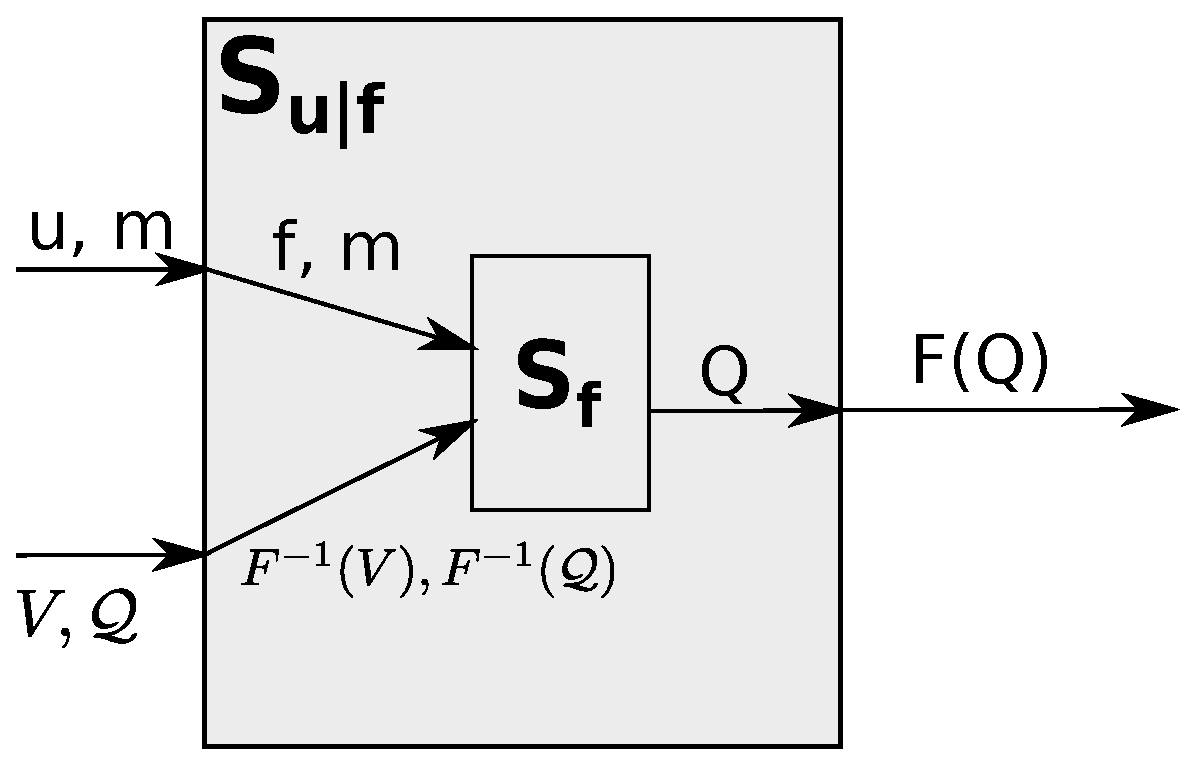
\includegraphics[width=.45\linewidth]{figures/S-f-to-u}
    \label{fig:S-t-to-u}
  }
  \subfigure[Construct $S_{f|u}$ from $S_u$]{
    \includegraphics[width=.45\linewidth]{figures/S-u-to-f}
    \label{fig:S-u-to-f}
  }
  \caption{These two figures illustrates how to construct a strategy for
  uniform PDF $u$ from another strategy for another arbitrary PDF $f$ and vice
  versa. Here we depict a strategy as a box which takes four inputs $f, m, V,
  \mathcal Q$ (PDF, number of unknown values, reported values set, set of asked
  queries) and make an output $Q$ (the next query)} \label{fig:uniform}
\end{figure}

After that, we prove that descending queries are optimal for this best
case optimizing problem.

\begin{lemma}\label{lemma:descending}

There exists an optimal strategy with only descending queries
$Q_1 = [q_1, 1], ~Q_2 = [q_2, q_1), ~Q_3 = [q_3, q_2)\ldots$

\end{lemma}

\begin{proof}

If not, there must be an optimal strategy where none of its
non-descending queries can be changed to descending queries without increasing
the cost. In that strategy $S$, there must be a first non-descending query
$Q_{i+1} = S\big(F, m, V, \mathcal Q = \{Q_1, Q_2, \ldots, Q_i\}\big)$ where
$Q_1$ to $Q_i$ are all descending.  We can make another descending query
$Q'_{i+1} = [q'_{i+1}, q_i)$ (or $Q'_{i+1} = [q'_{i+1}, 1]$ if $i = 0$) such
that
\[
\Pr(v \in Q_{i+1}) = \int \limits_{Q'_{i+1}} f(x) \mathrm d x = \int \limits_{Q_{i+1}} f(x) \mathrm d x = \Pr(v \in Q'_{i+1})
\]
After $Q'_{i+1}$, we'll use as optimal query as
possible.

Since $Q_1$ to $Q_i$ are all descending, we have $m = n$ and $V = \emptyset$ (otherwise
the strategy should terminate without asking $Q_{i+1}$).
Define $C$ to be the expected cost of using $Q_{i+1}$ and later queries. Similarly we define $C'$ for $Q'_{i+1}$:\\
$
C = b + \sum_{j=0}^n p_j ( j \cdot c + C_j)
$
and
$
C' = b + \sum_{j=0}^n p'_j ( j \cdot c + C'_j)
$
where:
%\begin{enumerate}
%\item 
$p_j$ (or $p'_j$) is the probability that there are $j$ reported values within $Q_{i+1}$ (or $Q'_{i+1}$);
%\item 
$C_j$ (or $C'_j$) is the expected cost of later queries given that $j$ values have been
found in $Q_{i+1}$ (or $Q'_{i+1}$).
%\end{enumerate}

As $\Pr(v \in Q_{i+1}) = \Pr(v \in Q'_{i+1})$, we have $p'_j = p_j$. Since $Q'_{i+1}$ is a
descending query, $\forall j > 0, ~C'_j = 0 \leq C_j$. And by lemma \ref{lemma:uniform},
$C'_0 = C_0 = C^*(n)$ because knowing no value is in $Q_1, Q_2, \ldots, Q_{i+1}$ is equivalent
to revise PDF $f(x)$ to a refined PDF 
\[
f_{i+1}(x) = \begin{cases}
	\lambda f(x), & x \notin Q_1 \cup Q_2 \cup \ldots \cup Q_{i+1} \\
	0, & x \in Q_1 \cup Q_2 \cup \ldots \cup Q_{i+1}
\end{cases}
\]
where $\lambda$ is a constant to make $\int_0^1 f_{i+1}(x) dx = 1$.

Thus $C' \leq C$ which contradicts to that no non-descending query can be changed to
descending query without increasing the cost.

\end{proof}

Finally, we conclude the optimality of MVAs.

\begin{theorem}\label{theorem:MVA_eq}

Among all mechanisms that can include multiple rounds of broadcasts and are
required to be efficient (allocate the item to the bidder with highest
valuation), Multi-round Vickrey Auctions (MVAs) are of minimum cost.

\end{theorem}

\begin{proof}

The best case optimizing problem defined in definition \ref{def:query} provides
us a lower bound of minimum cost we can achieve by any mechanisms.  By lemma
\ref{lemma}, such lower bound minimum cost can be achieved by descending query
strategy $Q_1 = [q_1, 1], Q_2 = [q_2, q_1), Q_3 = [q_3, q_2) \ldots$.  Making
$a_1 = q_1, a_2 = q_2, a_3 = q_3, \ldots$, by theorem \ref{theorem:MVA_eq} we
are able to design such an MVA with reserve prices $r_1, r_2, \ldots$  whose
Bayesian Nash Equilibrium achieves this best case descending query strategy.
Thus, MVAs are optimal.

\end{proof}

And by revenue equivalence theorem, MVAs maximize the seller utility.

\begin{corollary}

If all broadcast costs and bidding costs are charged to sellers, MVAs are
optimal if efficiency is required.  Such optimal MVA is the one that minimizes
the overall cost.

\end{corollary}

\subsection{Cost Minimized $\alpha$-MVA}

\subsection{Approximation of $\alpha$ and Experiments}

It's difficult to get an exact closed formula for optimal $\alpha$. Thus we are
going to use a closed formula to approximate this $\alpha$. We'll conduct
experiments to compare our approximation with the optimal $\alpha$ that's
computed numerically. We are also going to show comparisons between optimal
MVA, approximate optimal MVA and other conventional mechanisms such as Vickrey
auctions.


